\documentclass{standalone}

\usepackage{tikz}
\usepackage{tkz-euclide}
\usetikzlibrary{calc}
\usetikzlibrary{positioning}
\usetikzlibrary{arrows.meta}

\usepackage{times}


\begin{document}
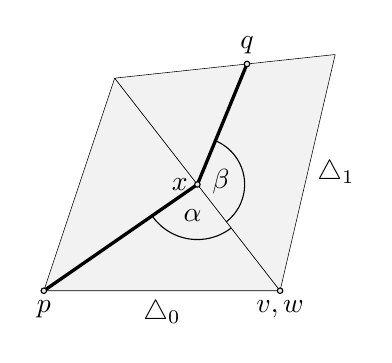
\begin{tikzpicture}[%
  >={Stealth[scale=1.0]},
]

  \tkzDefPoint(0.0, 0.0){A}
  \tkzDefPoint(3.0, 0.0){B}
  \tkzDefPoint(0.9, 2.7){C}
  \tkzDefPoint(3.7, 3.0){D}

  \tkzDefShiftPoint[A](0,0){p}

  \tkzDefPointOnLine[pos=0.5](B,C)
  \tkzGetPoint{x}

  \tkzDefPointOnLine[pos=0.6](C,D)
  \tkzGetPoint{q}

  \tkzDrawPolygon[color=black,fill=black!5](A,B,C)
  \tkzDrawPolygon[color=black,fill=black!5](B,C,D)

  \tkzMarkAngle[size=0.7](p,x,B)
  \tkzLabelAngle[pos = 0.4](p,x,B){$\alpha$}

  \tkzMarkAngle[size=0.6](B,x,q)
  \tkzLabelAngle[pos = 0.3](B,x,q){$\beta$}

  \tkzDrawSegments[very thick](p,x x,q)

  \tkzLabelSegment[below](A,B){$\triangle_0$}
  \tkzLabelSegment[right](B,D){$\triangle_1$}

  \tkzDrawPoints(p,x,q,B)
  \tkzLabelPoint(p){$p$}
  \tkzLabelPoint[left](x){$x$}
  \tkzLabelPoint[above](q){$q$}
  \tkzLabelPoint(B){$v,w$}

\end{tikzpicture}
\end{document}
